\documentclass{beamer}
\usetheme{Boadilla}

\usepackage{tikz}
\usepackage{soul}


\title{SAT Solving with Conflict Driven Clause Learning}
% \subtitle{Overview and Implementation}
\author{William Schultz}
\institute{CS 7240 Final Project}
\date{\today}

\begin{document}

\newcommand{\green}[1]{\textcolor{green}{#1}}
\newcommand{\red}[1]{\textcolor{red}{#1}}

\begin{frame}
    \titlepage
\end{frame}

\begin{frame}{Overview and Project Goals}
\begin{itemize}
    \item Satisfiability is the canonical NP-complete problem.
    
    \item Much work has been devoted to building efficient SAT solvers over last decades.\\
    
    \item \textbf{Project Goal:} Implement a basic SAT solver based on \textit{conflict driven clause learning} (CDCL), the dominant core technique used in modern solvers.
    \begin{itemize}
        \item Gain a deeper understanding of the DPLL and CDCL based algorithms for SAT solving
        \item Use as a platform for potentially exploring new SAT solving techniques 
        \item E.g. learning heuristics using a data-driven approach, extending methods of \textit{CrystalBall} \cite{2019sooscrystalball}
    \end{itemize}
\end{itemize}
\end{frame}

\begin{frame}{Review: The SAT Problem}
    The SAT problem:
    \vspace{12pt}

    \textit{Given a boolean formula in conjunctive normal form (CNF), determine whether there exists an assignment to the variables of the formula that makes the overall formula true.}

    \pause
    \vspace{12pt}
    e.g.
    \begin{align*}
        (x_1 \vee x_2) \wedge (\neg x_3 \vee \neg x_1)
    \end{align*}
    \pause
    \begin{center}
        SAT, with $\{x_1=1,x_2=0,x_3=0\}$. 
    \end{center}
    \pause
    CNF notation:
    \begin{align*}
        \{\{x_1, x_2\}, \{\neg x_3, \neg x_1\}\}
    \end{align*}
\end{frame}

\begin{frame}{DPLL: SAT as Search}
    \begin{itemize}
        \item A basic approach to solving SAT is to view it as a search problem over possible assignments.
        \item This is the basis of the Davis–Putnam–Logemann–Loveland (DPLL) algorithm \cite{dpll1961}
        \item Basic idea of DPLL is to do a depth first, brute force search with backtracking along with some basic formula simplification as you go.
        \begin{itemize}
            \item Also employs the \textit{unit propagation rule}
        \end{itemize}
    \end{itemize}
\end{frame}

\begin{frame}{Unit Propagation}
    \begin{itemize}[<+->]
        \item Core simplification rule employed in DPLL, and also in CDCL as we will see later.
        \item A \textit{unit clause} is a clause that contains exactly one literal.
        \item If a CNF formula contains a unit clause then we can apply unit propagation i.e. set that literal to the appropriate truth value to satisfy its clause e.g.
        \begin{align*}
            \action<+->{
                &\{\{b\}, \{\neg b, \neg c\}, \{c, \neg d\}\}\\
            }
            \action<+->{
                &\{\{\green{b}\}, \{\red{\neg b}, \neg c\}, \{c, \neg d\}\}\\
            }
            \action<+->{
                &\{\{\neg c\}, \{c, \neg d\}\} \\
            }
            \action<+->{
                &\{\{\green{\neg c}\}, \{\red{c}, \neg d\}\}\\
            }
            \action<+->{
                &\{\{\neg d\}\}\\
            }
            \action<+->{
                &\{\{\green{\neg d}\}\}\\
            }
            \action<+->{
                &\{\} \quad (\text{SAT})
            }
        \end{align*}
    \end{itemize}
\end{frame}

\begin{frame}{DPLL: Example}
    \begin{columns}
        % CNF formula.
        \begin{column}{0.45\textwidth}
            \begin{align*}
                &\{\only<1-2>{\neg a}\only<3->{\red{\neg a}},
                   \only<1-3>{b}\only<4->{\green{b}}\}\\
                &\{\only<1-3>{\neg b}\only<4->{\red{\neg b}},
                   \only<1-4>{\neg c}\only<5->{\green{\neg c}}\} \\
                &\{\only<1-4>{c}\only<5->{\red{c}},
                   \only<1-5>{\neg d}\only<6->{\green{\neg d}}\}\\
            \end{align*}
            \only<0-3>{\phantom{unit propagate}}\only<4>{unit propagate $b$}\only<5>{unit propagate $\neg c$}\only<6->{unit propagate $\neg d$}
        \end{column}

        % DPLL search tree.
        \begin{column}{0.45\textwidth}
            % \begin{center}
            \begin{tikzpicture}
    \node {a}
    child [] {node {b} 
        child [] {node {\only<1->{c}}
            child [] {node {d} 
                child [] {node {x} edge from parent [] node [left]{1}}
                child [] {node {x} edge from parent [] node [right]{\only<1-5>{0}\only<6->{\textbf{0}}}}
            edge from parent [] node [left]{
                \only<1-4>{0}\only<5->{\textbf{0}}
            }} 
        edge from parent [] node [left]{\only<1-3>{1}\only<4->{\textbf{1}}}}
        child [] {node {c} 
        edge from parent [] node [right]{0}}
    edge from parent [] node [left]{\only<1-2>{1}\only<3->{\textbf{1}}}}
    child [] {node {b} 
    edge from parent [] node [right]{0}};
\end{tikzpicture}
            % \end{center}
        \end{column}
    \end{columns}
\end{frame}

\begin{frame}{Beyond DPLL: Learning from Conflicts}
    \begin{itemize}[<+->]
        \item DPLL is a relatively naive algorithm
        \item An extension to this basic framework is to \textit{learn from conflicts} 
        \item When you encounter a conflict in the search tree, \textit{learn} a clause that prevents you from making the similar mistakes again
        \item This fundamental approach is known as \textit{conflict-driven clause learning} (CDCL) and started being employed in SAT solvers around the late 90s and early 2000s.
        \item In addition, employ \textit{non-chronological backtracking}
    \end{itemize}
\end{frame}

% \begin{frame}{CDCL}
% \begin{itemize}
%     \item When using CDCL, if a conflict is encountered, we not only backtrack to the previous level, as in DPLL
%     \item We try to learn a \textit{conflict clause} along with a \textit{backjump} level, which determines how far back in the search tree to unwind to.
% \end{itemize}
% \end{frame}

\begin{frame}{CDCL Example}

    \begin{columns}
        % CNF formula.
        \begin{column}{0.25\textwidth}
            \begin{align*}
                &\{a,b\}\\
                &\{b,c\}\\
                &\{\neg a, \neg x, y\} \\
                &\{\neg a, x, z\} \\
                &\{ \neg a, \neg y, z\} \\
                &\{ \neg a, x, \neg z\} \\
                &\{ \neg a, \neg y, \neg z\}
            \end{align*}
        \end{column}

        % DPLL/CDCL search tree.
        \begin{column}{0.65\textwidth}
            \begin{figure}
                \begin{tikzpicture}
    \node {$a$} [sibling distance = 2.9cm]
    child [] {node {
            \only<1->{$b$}
            % \only<3->{\textcolor{blue}{b}}
            } [sibling distance =3.65cm]
        % c=1
        child [] {node {\only<1->{$c$}} [sibling distance = 1.75cm]
            child [] {node {$x$} [sibling distance = 1.15cm]
                child [] {node  {\only<1-2>{\red{X}}\only<3->{\textbf{\red{X}}}} edge from parent [] node [left]{
                    \only<1-2>{1}\only<3-7>{\textbf{1}}\only<8-9>{1}\only<10-12>{\textbf{1}}\only<13->{1}
                }}
                child [] {node {\red{X}} edge from parent [] node [right]{0}}
            edge from parent [] node [left]{
                \only<1-2>{1}\only<3-7>{\textbf{1}}\only<8->{1}
            }} 
            child [] {node {$x$} [sibling distance = 1.15cm]
                child [] {node  {\red{X}} edge from parent [] node [left]{1}}
                child [] {node {\red{X}} edge from parent [] node [right]{0}}
            edge from parent [] node [right]{0}}
        edge from parent [] node [left]{
            \only<1-2>{1}\only<3-7>{\textbf{1}}\only<8->{1}
        }}
        % c=0
        child [] {node {$c$} [sibling distance =1.75cm]
            child [] {node {x} [sibling distance = 1.15cm]
                child [] {node {\red{X}} edge from parent [] node [left]{1}}
                child [] {node {\red{X}} edge from parent [] node [left]{1}}
            edge from parent [] node [left]{1}}
            child [] {node {x} [sibling distance = 1.15cm]
                child [] {node {\red{X}} edge from parent [] node [left]{1}}
                child [] {node {\red{X}} edge from parent [] node [left]{1}}  
            edge from parent [] node [right]{0}}
        % edge from parent [] node [left]{0}} 
        edge from parent [] node [right]{0}}
    edge from parent [] node [left]{\only<1-2>{1}\only<3-7>{\textbf{1}}\only<8>{1}\only<9-13>{\textbf{1}}\only<14->{1}}}
    % a = 0.
    child [] {node {$b=1$\, $\{\}$ \green{sat}} 
    edge from parent [] node [right]{\only<1-13>{0}\only<14->{\textbf{0}}}};
\end{tikzpicture}
                \caption{Termination tree using standard DPLL.}
            \end{figure}
            % \begin{center}
            % \end{center}
        \end{column}
    \end{columns}
\end{frame}

\begin{frame}{CDCL Example}
\begin{itemize}
    \item From basic DPLL traversal we can see that there is no satisfying assignment where $a=1$
    \item But, we could have learned earlier on that this was an unfruitful section of the search space
    \item Idea is to analyze the conflict the occurred from partial assignment $\{a=1,b=1,c=1,x=1\}$
\end{itemize}
\end{frame}

\begin{frame}{CDCL: Implication Graph}
    \begin{itemize}
        \item Can represent the propagation of variable assignments in an \textit{implication graph}
        \item Nodes of this graph represent variable assignments made in the current search path
        \item Edges correspond to dependencies between these assignments.
\end{itemize}
\end{frame}


\begin{frame}{SAT Solver Implementation}
    \begin{itemize}
        \item Iimplementing my own CDCL SAT solver as a framework for exploring future potential SAT enhancements
        \item Around 1500 lines of C++, tested on a variety of easy to medium SAT benchmark problems
        \item \url{https://github.com/will62794/mysat}
    \end{itemize}
\end{frame}

\begin{frame}{Evaluation}
    \begin{itemize}
        \item Some peformance results of my SAT solver against a performant, modern solver.
    \end{itemize}
\end{frame}

\begin{frame}{Future Extensions and Learning Heuristics}
    \begin{itemize}
        \item Modern CDCL based SAT solvers employ many heuristics
            \begin{itemize}
                \item Variable ordering
                \item Clause deletion policies
            \end{itemize}
        \item Often these are ``expertly tuned'' heuristics
        \item \textit{CrystalBall} \cite{2019sooscrystalball}: Possible to learn better heuristics from data on SAT solver executions? 
    \end{itemize}
\end{frame}

\begin{frame}
    \begin{itemize}
        \item CrystalBall
    \end{itemize}
\end{frame}

% \begin{frame}{Future Extensions and Learning Heuristics}
%     \begin{itemize}
%         \item Resolution proofs
%         \item Variable ordering heuristics
%         \item Learning heuristics
%         \item Learning end to end SAT solver (neuroSAT)
%     \end{itemize}
% \end{frame}

\begin{frame}{}
    \begin{center}
        \Large
        Questions?
    \end{center}
\end{frame}

\bibliographystyle{alpha}
\bibliography{../references}

\end{document}

